\section{ Key Ideas and Architecture}
\label{sect:arch}


%\begin{figure}[htbp]
%  \centering
  %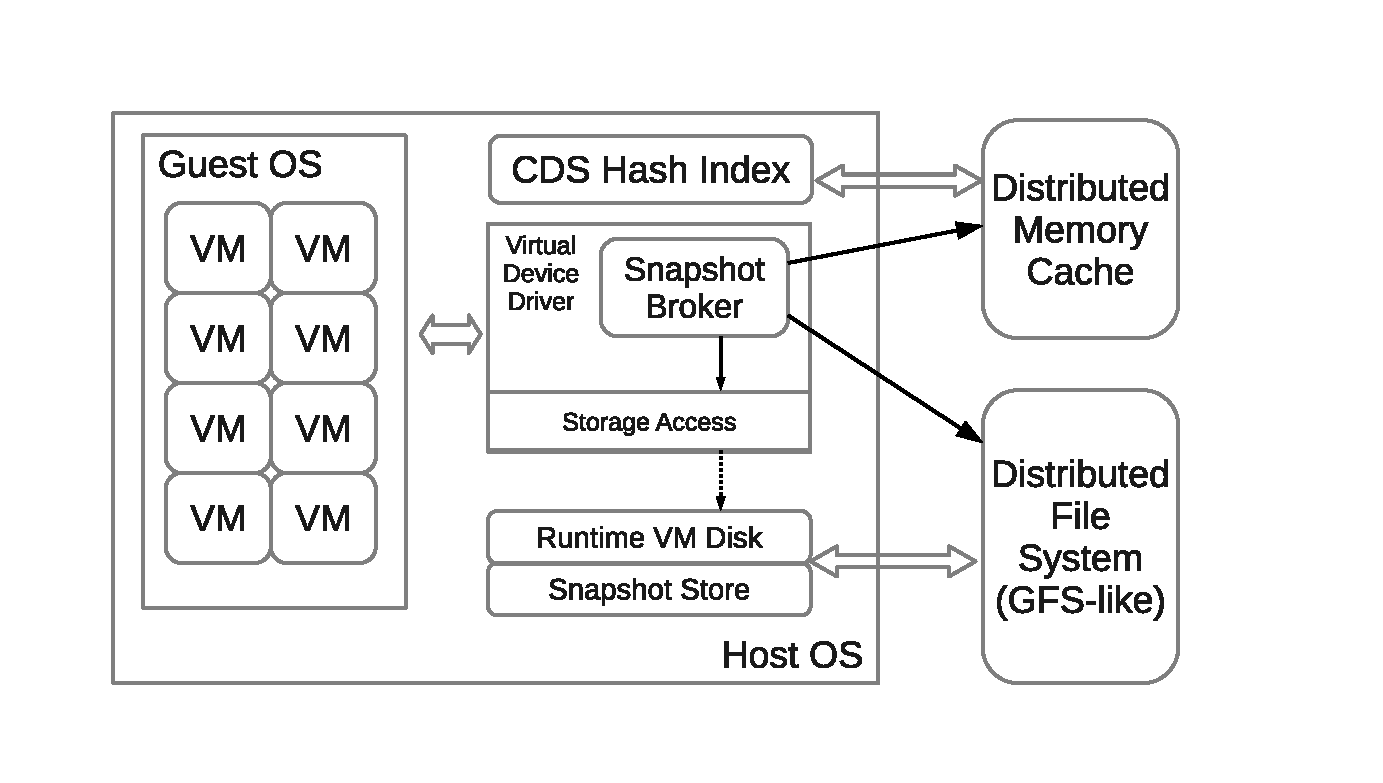
\epsfig{file=images/arch.eps, height=2in, width=2.66in}
%  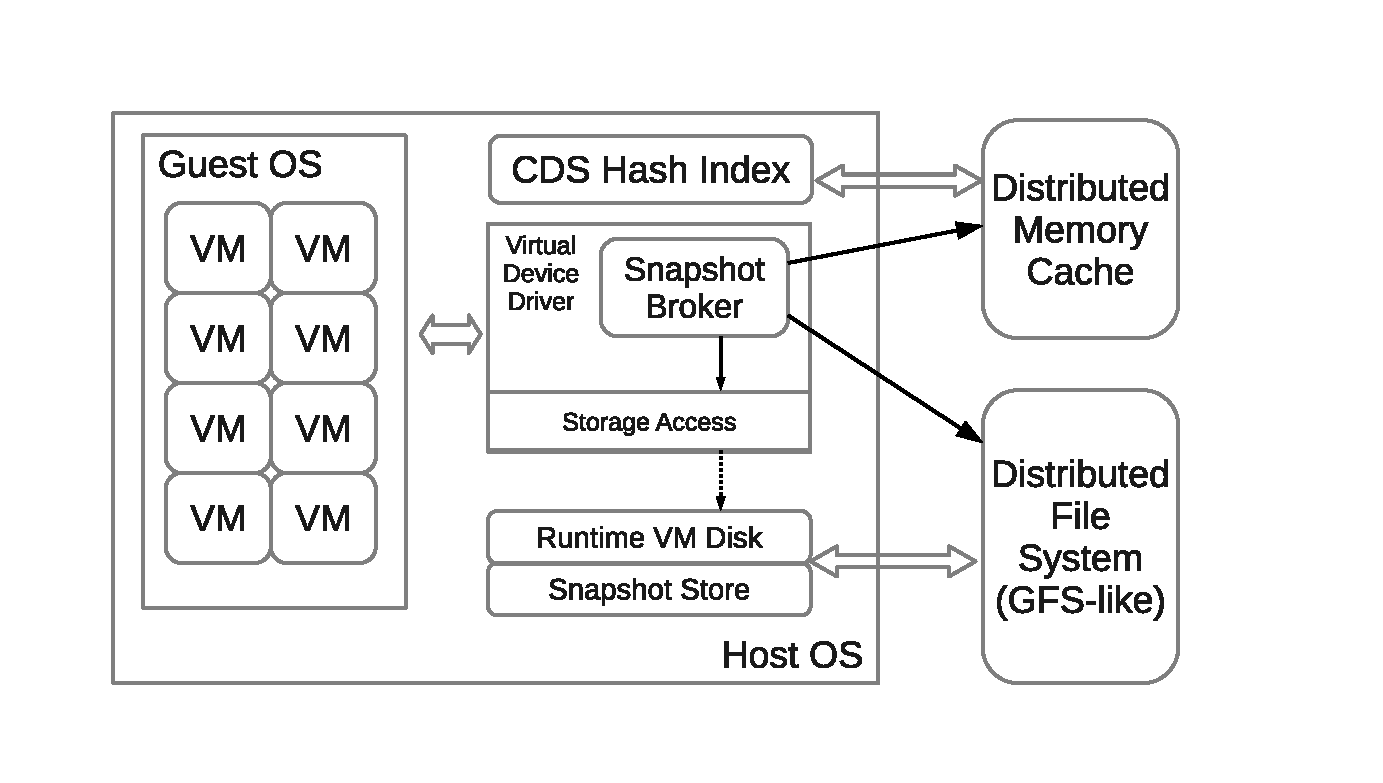
\epsfig{file=images/arch.eps, width=3.9in}
%  \caption{Snapshot backup architecture of each node.}
%  \label{fig:arch}
%\end{figure}


We consider deduplication in two levels. The first-level of data deduplication can be accomplished efficiently and 
inexpensively using a coarse-grain segment-level  dirty bit based detection in the OS level  to 
identify version difference from the previous snapshot to the current snapshot.  
Version-based detection has been used in the previous work~\cite{Clements2009,Vrable2009,TanIPDPS2011} and
we emphasize a segment-level coarse-grain setting to reduce the efforts in detection and maintaining dirty bits. 
Our experiment with Alibaba''s production dataset shows that over 70 percentage of 
duplicates can be detected using segment-based dirty bits while the segment size is as large as 2M bytes.  
This setting requires OS to keep the metadata for segment dirty bits and the amount of space for such segment 
dirty bits is negligible. In the second level of deduplication, remaining content blocks of each VM 
are compared with the signatures of all unique  blocks stored in the previous snapshots.

Our key ideas are summarized as follows.
\begin{itemize}


\item {\bf Separation of duplicate detection and data backup.}
%Request accumulation and partition-based deduplication.}
The second level duplicate detection requires a global comparison of 
content fingerprints of stored chunks with the new chunks scanned during 
the backup process. Bloom filters and caching allows some of content 
fingerprints to be stored on the cheap disks~\cite{bottleneck08}. Such an optimization is good 
for inline deduplication where chunks scanned need to be determined to be duplicate or not instantly without 
waiting while  it memory consumption is still significant in competing with stand virtual 
machine activities.  Our idea is to perform duplicate detection first before actual data backup.
That requires a pre-scanning of  data  blocks of VM images and after that, real backup  for those non-duplicates
is conducted. That does incur an extra  round of I/O reading for non-duplicate blocks while avoiding inline 
deduplication and leading to a much smaller resource requirement. 
During duplicate detection phase, detection requests can be accumulated on the disk 
for a period time  in a  partitioned manner.  Aggregated duplicate requests can be processed partition by partition. 
%We also accumulate the delete requests and perform them partition by partitions. 
Since each partition corresponds to a small portion of global content index, the cost to 
process requests within a partition is significant smaller than process all the requests globally.

\item {\bf Buffered data redistribution in parallel duplicate detection}.  
We let {\em global index} be the meta data containing the fingerprint values of all unique blocks
in the entire cluster and  the reference pointers which lead to the actual location of raw data.
A duplicate detection request for a content block needs to be compared with the global index to determine if this
block is non-duplicate. If it is a duplicate, return the corresponding reference pointer.
We conduct parallel processing of detection requests in all machines in a cloud cluster.
A logical way to distribute detection requests is to partition based on the content  hashing of data blocks
and the global index can also be partitioned accordingly in a  disjointed manner.
Initial data follows the VM distribution among machines and the detected results 
represented as  duplicate summary need to be collected following VM distribution. 
Therefore, there are two all-to-all data remapping operations involved.
One is to map detection requests from VM-based requests to the fingerprint based distribution.  
One is to map duplicate summary from fingerprint-based requests to the VM based distribution.  
The redistributed data needs to be accumulated on the disk to minimize the use of memory.
To minimize the cost of disk seek, outgoing or incoming data exchange messages need to be buffered to bundle small messages.
Given there are $p\times q$ partitions where $p$ is the number of machines and $q$ is the number of fingerprint-based partitions
at each machine, the number of buffers is big and space per each buffer  is small given the memory constraint.
Then there will be a large number of storage  IO operations involved, suffering the huge seek overhead.
We have designed an efficient data exchange and disk data buffering  scheme to address this.

%As we detect and backup requests before actual backup takes place,  we need to store chunk data on 
%temporary disks and once duplicates 
%are detected, we only need to fetch and store these non-duplicates 
%in the backup storage.  To minimize the storage usage of temporary disk space, we donot save the data content 
%of accumulated requests with replication, but we store  data separately for each virtual machine. In an event 
%that the storage of temporary accumulation fails for certain virtual machines, rescanning of these virtual machine images 
%is conducted and backup of these machines is re-initiated.   Meta data such as content hash for accumulated requests 
%is stored separately since we map the meta data into a set of buckets using chunk fingerprints. 
%The benefit of separating content and meta data is to allow fast recovery of backup operations while enabling bucket-based lazy deduplication.

\end{itemize}


We assume a flat architecture in which  all $p$ machines that host VMs in a cluster can 
be used in parallel for deduplication. 
The non-duplicate snapshot blocks are stored either in a distributed file system built on
this cluster  or in another  external storage system. 
We assume that  a small amount of local disk space and memory on each machine can be used 
to store global index and request accumulation.
%Our design is to minimize the usage of local memory and storage on each machine.


%While we assume all machines can process  independent or coordinated
%deduplication and backup operations in parallel,  
%our scheme uses a single-thread procedure on each machine to minimize the use of CPU, network bandwidth, and disk bandwidth.
\subsection{Data Structure}

\begin{figure}
\centering
\includegraphics[width=0.45\textwidth]{snapshopdata.pdf}
\caption{ Metadata structure of a VM snapshot.}
\label{fig:snapshot}
\end{figure}

The representation of each snapshot saved in the backup storage
has a two-level level index data structure in the form of a hierarchical
directed acyclic graph as shown in Figure~\ref{fig:snapshot}.
An VM image is divided into a set of segments and each  segment contains hundreds of content blocks from the bottom level.
These blocks are of variable-size, partitioned using
the standard chunking technique~\cite{similar94} with 4KB as the average block size. 
%To simplify the deduplication process, segments are aligned to fix-sized boundaries, currently using 2MB.

Segment metadata (called segment recipe) records its  content block hashes and data pointers. 
The snapshot recipe contains a list of segments and other meta data information.
If a segment is not changed from one snapshot to another, indicated by a dirty bit embedded in the virtual disk driver, 
its content blocks are not changed as well, thus its segment recipe contains a reference pointer to an earlier segment.
If a block is duplicate to another block in the system,  the block recipe contains a reference pointer to an earlier block.


\subsection{Processing flow and resource usage}

The data flow of our partition-based  duplicate detection is depicted in
Figure~\ref{fig:flow}. 
%let $v$ be the total number of virtual machines hosted in  a cluster,  
%we divide the backup into $k$  iterations. 
\begin{figure}
\centering
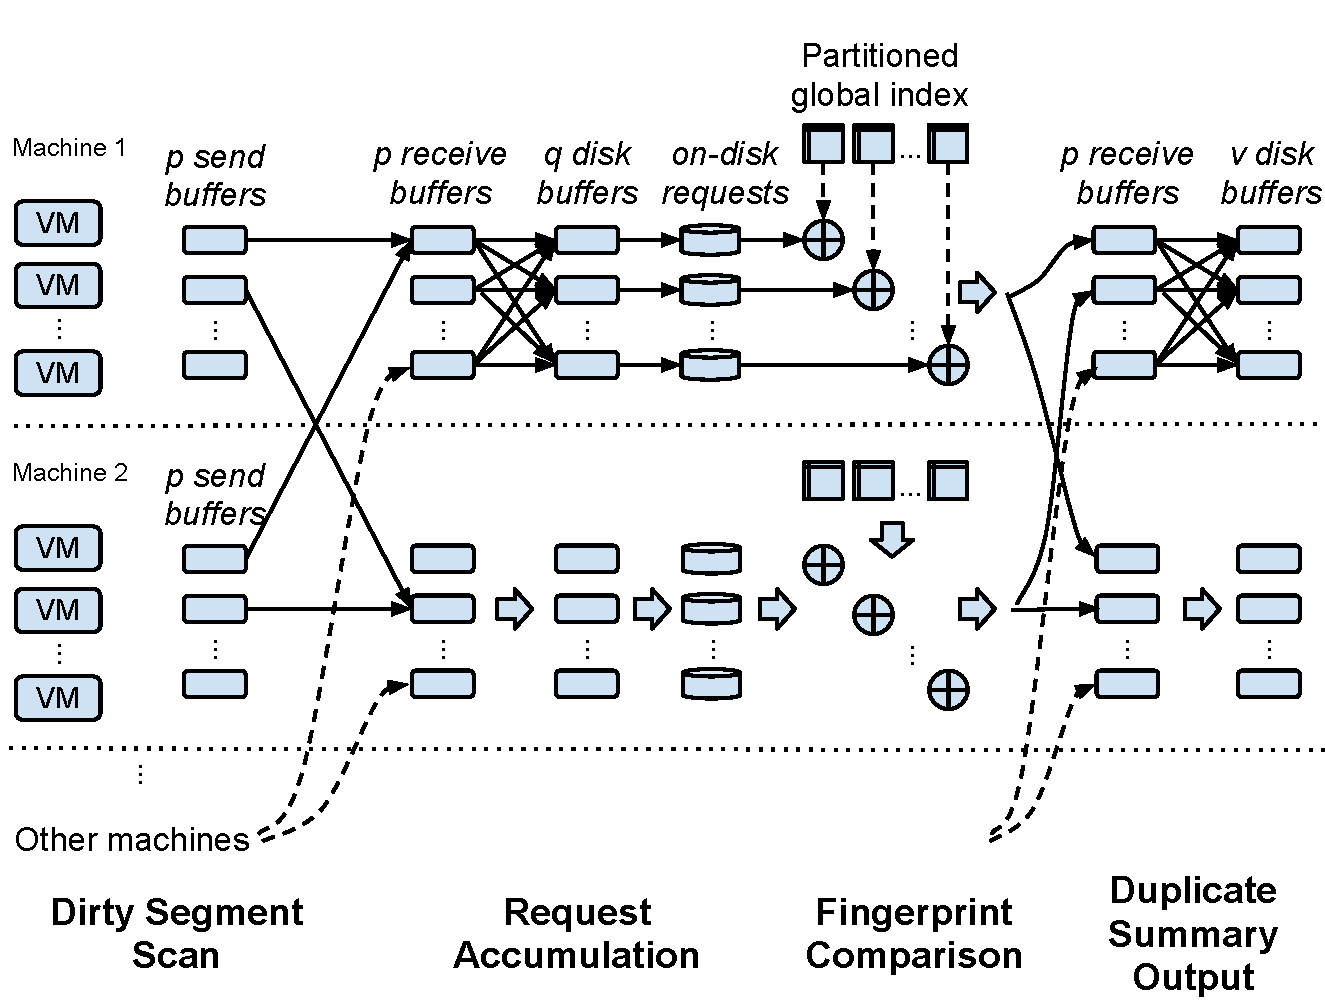
\includegraphics[width=0.45\textwidth]{steps.pdf}
\caption{ Processing steps of duplicate detection.}
\label{fig:flow}
\end{figure}

\begin{itemize}
\item
The first step is that each machine independently reads  
%$v/k$  
virtual machine images that need a backup
and forms duplicate  detection requests. For those segments that have been modified since last backup indicated by 
dirty bits,  the system divides  each segment into a sequence of chunk blocks,  computes the meta 
information such as chunk fingerprints,  sends the metadata of a chunk block, and accumulate  into 
a partition bucket on the temporary disk storage. 
The partition mapping is using a hash function applied to the content fingerprint. 
Assuming all machines have a  homogeneous resource configuration, each machine is evenly  assigned with
$q$ parititons of content hash and accumulates corresponding requests on the disk. 
There are two options to assign buffers in each machine to buffer requests for each partition.
1) Each machine has  $p\times q$ send buffers corresponding to $p\times q$ partitions in the cluster
since any content block in a VM image of this machine can be sent to any of these partitions.
2) Each machine has $p$ receive buffers correspond to $p$ machines in the cluster and $q$ receive 
buffers to temporarily accumulate messages from other machines, and then output each buffer to the local disk
when it becomes full.  Option 2 is much more efficient than Option 1 because $p+q$ is much smaller than
$p\times q$, as a result each buffer has a bigger size to accumulate data and results in 
much less disk seek overhead.

%We assume that the startup cost for network message sending is  much more less (e.g. an order of magnitude
%less) than from one machine to another 
%disk storage startup cost such as seek is much mu
%Note that we only accumulate requests with their meta data information.
\item
The second step is to perform duplicate detection for  all requests accumulated in the partitions.  
The system maintains the index of all chunk fingerprints divided in the buckets. We load the global index partition 
and accumulated corresponding requests, and compare them to  identify the duplicated blocks.  
Then we unload them, load the global index and accumulated requests for another partition. 
This process is repeated until all buckets are processed.

As chunk blocks are detected as duplicates, the meta information on duplicates is 
remapped from fingerprint-based distribution  to VM-based distribution. In this way, duplicate information 
for segments of each VM is collected in one place, which will be used in next step. 
In the sending side, each machine scans identified duplicates for one target machine,
and then scans for another machine. In this way, it sends duplicate summary to the corresponding machines one by one
to minimize the startup cost for sending a message.
In the receiving side, 
%All-to-all machines data exchange is conducted  so that  
each machine allocates $q$ receive buffers corresponding to
$q$ local partitions, to hold received messages from other machines.  
When a receive buffer for a VM is  full, the data is written to the local disk storage. 
%These substeps are repeated as the stream of data is exchanged when each machine compares through all $q$ partitions.

\item The third step is to read  non-duplicate blocks from each VM and output to the final backup 
storage. Additionally, the global index on each machine is updated with the meta data of new chunk blocks added.
In this process, if a segment is not dirty, we only need to output the segment meta data 
such as reference pointers to the original segments previously saved in the backup.  
If a segment is dirty,  we use the duplicate summary information from Step 2 for internal 
duplicate blocks of this dirty segment and output the remaining non-duplicate blocks to the backup storage.
\end{itemize}

%          In fetching non-duplicates,    it is sometime faster that we fetch a large number of consecutive chunk blocks from an accumulated  segment which contains duplicated chunks,  to avoid the random seek overhead.


The above steps can be executed by each machine
using one thread to minimize the use of CPU, network bandwidth, and disk bandwidth.
The  disk storage usage on each machine 
is fairly small for  storing part of global index and
accumulating  duplicate detection requests that contain fingerprint information.   
We impose a limit for memory allocated at each machine node to accomplish low-cost deduplication.  
Memory usage for each step of above scheme is carefully controlled as follows.
\begin{itemize}
\item For Step 1, the allocated memory for each machine is evenly divided for $p$ send buffers and $q$ receive buffers.

%1) $p$ send buffers. images, sends the fingerprint of a dirty block to a machine that is responsible for this fingerprint.
%2) Buffer requests gathered from other machines and divide those requests into $q$ buckets. Once a buffer for each bucket is full, output to the disk storage.
\item 
For Step 2,  the allocated memory serves 2 purposes. 1) Space for hosting a partition of global index and 
the corresponding partition of  deduplication requests. 2) Buffer space for $q$ receive buffers.
%%accumulating duplicate summary for each targeted VM.   Once  each machine processes a bucket of  duplicate detection requests, 
The duplicate summary sent other machines and acclimated for each VM contains
the block ID and  the reference pointer.   
%For each machine which hosts $v$  VMs, and will receive messages from many other machines, 
%the system needs to allocate buffer space for each VM ot accumulate the duplicate summary records. 
%When a buffer for a VM is full, the result is written to the disk.

\item For Step 3 to  perform the real backup for each VM, 
memory is used to hold the meta information summary of all duplicate blocks obtained  from Step 2. 
Another memory usage is to fetch a sequence of blocks from a virtual machines (most of them are non-duplicate) 
and write them to the  backup storage.

\end{itemize}
%We find the memory for step 2 is most critical for buffering duplicate summary in hiding the latency. 
%Certainly most storage system can allow many IO requests issued in parallel overlapping the IO latency.  
%Here we assume the worst case and also minimize the IO bandwidth usages by issuing 
%one request at a time to use the minimal disk bandwidth resource.

{\bf Snapshot deletion.} Each virtual machine will keep at most $x$ snapshots of VM images and thus
expired snapshots will be deleted unless its owner explicitly asks for its retention. 
A block or the entire segment can be deleted if its reference counter is zero.
%As we discussed in Section~\ref{sect:data}, the reference counter is kept in the global index, partitioned among machines. 
We periodically read all receipts of active 
snapshots and compute the counter of all blocks while still following the fingerprint-based partitioning.
That is based on the idea of mark-and-sweep~\cite{MarkSweep} while 
we deal such snapshot deletion in three partition-based steps similar to the VM snapshot backup.
Step 1 is to read  the meta data of snapshots such as segment and block
recipes and  accumulate  reference count requests in different machines  in the fingerprint based distribution.
The second step  is to count references within each partition and detect those records with zero 
reference. The third step is that every VM gathers the confirmed deletion requests for its content and sends them
to the backup storage.
The archival data repository may log these deletion requests,  and will periodically perform a compaction operation when 
its deletion log is too big. 
%Due to the paper constraint, we will not discuss the deletion operations in details.

%The above method requires the counter information to be consistently maintained in the global index.
%Finally the deleteion summary. it will adjust the corresponding reference counts. At the end of bucket worker's operation, it outputs the unused blocks information to each VM data repository's deletion log.


%This compaction will make a copy of all the data in use, and remove the obsoleted blocks. However, after such a compaction, many block offsets will be changed, as a result, such changes are sent to the bucket job queue so that changes will be reflected upon the next bucket update.

%Since we maintain a single copy of each block information in the bucket index, and there is at most one bucket worker operating the bucket index at one time, it it safe to do the simple reference counting rather than mark-and-sweep.
